%%%%%%%%%%%%%%%%%%%%%%%%%%%%%%%%%%%%%%%%%%%%
\chapter{Background}
%%%%%%%%%%%%%%%%%%%%%%%%%%%%%%%%%%%%%%%%%%%%
\begin{center}
  \begin{minipage}{0.75\textwidth}
    \begin{small}
      “The interaction between material bodies can be described either by formuating the action at a distance between the interacting bodies or by separating the interaction process into the production of a field by one system and the action of the field on another system” .
      \emph{Classical Electricity \& Magnetism. Panofksy, Phillips}\\.
    \end{small}
  \end{minipage}
  \vspace{0.5cm}
\end{center}

%%%%%%%%%%%%%%%%%%%%%%%%%%%%%%%%%%%%%%%%%%%
\section{The Nature of Light and the Electromagnetic Spectrum}
%%%%%%%%%%%%%%%%%%%%%%%%%%%%%%%%%%%%%%%%%%%
Light is fundamental to life.  In Maxwell’s’ theory on light he explained how electromagnetic phenomenon can be expressed in terms of waves \cite{maxwell}.  These waves move at the speed of light.  The light that human eyes can detect is a small portion of the electromagnetic spectrum called ‘visible light’.
%
%CHECK [insert EM image here]
\begin{figure}[!htb]
    \begin{center}
        \makebox[\textwidth]{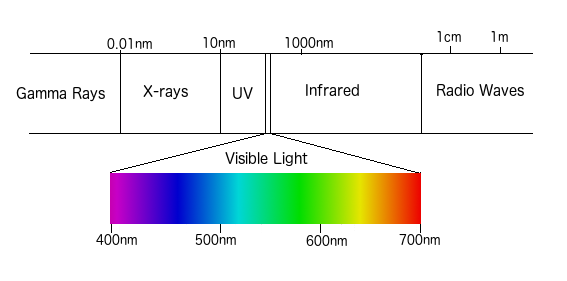
\includegraphics[scale=0.75]{/Sources/Background/Nature_of_Light/EM-spectrum.png}}
    \end{center}
    \caption{Electromagnetic Spectrum - Partial}
    \label{fig:polarization}
\end{figure}
Different frequencies of light correspond to different colors on the visible spectrum.  These waves are made up of two parts, the electric and magnetic.  Due to their similar nature often only the electrical portion is considered at first for mathematical simplicity.

The electrical portion of EM waves, and the only portion considered here, can be described as the sum of two sinusoidal waves representing the orthogonal x and y components in Cartesian space.
%
\begin{align}
    E(z,t)=E_x (t)+E_y (t)\\
    E_x (t)=E_{0x} cos( \theta+\delta_x )\\
    E_y (t)=E_{0y} cos( \theta+\delta_y )
\end{align}
%
where $ \theta = \delta t-kz $ is the wave propagator that determines the frequency and direction of propagation for the wave.$ \delta_y and \delta_x $ represent the phase delay for each component of the wave.

When more than one sine wave is considered, as in the case of EM waves, an overall phase delay between the them is considered and represented as $ \tau=\delta_y-\delta_x $.

Light can also be viewed as packets of energy known as photons.  The energy of photons is related to its frequency $v$ and a constant, known as Planck’s constant $h$ \cite{ecophysiology}.
%
\begin{align}
	h=6.62e-34 [m^2 kg/s]\\
	E=hv [Joules]
\end{align}
%
This simple equation shows that for higher frequencies, particles have higher energy.

%%%%%%%%%%%%%%%%%%%%%%%%%%%%%%%%%%%%%%%%%%%%%%%%%%%%%%%%%%%%%%
% Nature of Light Subsections
%%%%%%%%%%%%%%%%%%%%%%%%%%%%%%%%%%%%%%%%%%%%%%%%%%%%%%%%%%%%%%
%%%%%%%%%%%%%%%%%%%%%%%%%%%%%%%%%%%%%%%%%%%
\subsection{Polarization of EM Waves}
%%%%%%%%%%%%%%%%%%%%%%%%%%%%%%%%%%%%%%%%%%%
The polarization of EM waves is determined, for monochromatic frequencies, by the relative intensity and phase of their respective $x$ and $y$ components.  These relationships can be viewed as the path traced by the tip of the electric field vector when looking in the direction of illumination.  Common sources of illumination are lasers, light emitting diodes, halogen lamps, the sun, etc.

In its most general form, the polarization is referred to as being elliptical, and its $x$ and $y$ amplitudes, and phase delay can be described in the form of the polarization ellipse.

It has been shown that the form of the polarization ellipse can be derived from the solution to the plane wave equation for the electromagnetic wave.  Using the relationships defined in the previous section and defining,
%
\begin{align}
    \tau=\omega t-kz+\delta_x
\end{align}
%
We can then define the $x$ and $y$ component of the wave as
%
\begin{align}
	E_x (t)=E_{0x} cos(\tau)\\
	E_y (t)=E_{0y} cos(\tau+\delta_y )
\end{align}
%
The $y$ component is then separated using known trigonometric identities and equation
%
\begin{align}
E_y (t)=E_{0y} (cos(\tau) cos(\delta)-sin(\tau)sin(\delta))
\end{align}
%
[TODO show what delta equals here how delta y goes to just delta?]
Dividing each equation by its intensity results in
%
\begin{align}
    \frac{E_x (t)}{E_{0x}} =cos(\tau) \\
    \frac{E_y (t)}{E_{0y}} =cos(\tau+\delta_y )
\end{align}
%
Again using known trigonometric identities
%
\begin{align}
    \frac{E_y (t)}{E_{0y}} = \frac{E_x (t)}{E_{0x}}   cos(\delta)-\sqrt{1-\frac{E_x (t)^2}{E_{0x}^2} } sin(\delta)
\end{align}
%
Rearranging and squaring both sides results in
%
\begin{align}
    (\frac{E_x (t)}{E_{0x}}   cos(\delta)-\frac{E_y (t)}{E_{0y}} )^2=(\sqrt{1-\frac{E_x (t)^2}{E_{0x}^2} } sin(\delta))^2
\end{align}
%
The factorization of this equation can be rearranged into the standard form of an ellipse such that
%
\begin{align}
    \frac{E_x (t)^2}{E_{0x}^2} +\frac{E_y (t)^2}{E_{0y}^2} -2 \frac{E_x E_y}{E_{0x} E_{0y} } cos(\delta)=sin^2 (\delta)
\end{align}
%
And is graphed as
%[CHECK replace this image with one that has both parameters]
\begin{figure}[!htb]
    \begin{center}
        \makebox[\textwidth]{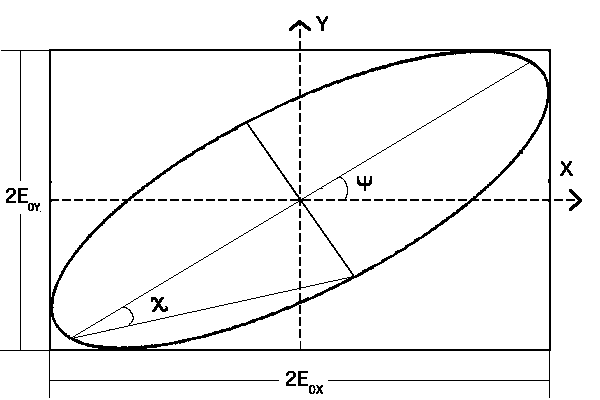
\includegraphics[scale=0.5]{/Sources/Background/Nature_of_Light/polarization-ellipse-binary-v2.png}}
    \end{center}
    \caption{Polarization Ellipse}
    \label{fig:polarization}
\end{figure}
%

Due to the restraints of modern optical sensors, it is not possible to directly measure the polarization ellipse, for a light beam, at any instant in time.  Taking the time average of the ellipse results in quantities that can measured by detectors in order to quantify the polarization state of an EM wave.  It is therefore necessary to derive parameters from the ellipse that can be measured.
Starting from the equation for the polarization ellipse, taking the time average of the E field results in
%
\begin{align}
    \frac{E_x (t)^2}{E_{0x}^2} + \frac{E_y (t)^2}{E_{0y}^2} - \frac{2 E_x (t) E_y (t)}{E_{0x} E_{0y} } cos(\delta)=sin^2 (\delta)
\end{align}
%
the time averages are calculated as [CHECK Fix this equation]
%
\begin{align}
    <E_x (t)^2> = lim_{T \rightarrow \infty} \int_{0}^{2\pi} E_{0x} cos(\tau)  d\tau=\frac{1}{2} E_{0x}^2
\end{align}
%
and similarly
%
\begin{align}
    <E_y (t)^2>  = \frac{1}{2} E_{0y}^2 \\
	<E_x (t) E_y (t)>  =  \frac{1}{2} E_{0x} E_{0y} cos(\delta)
\end{align}
%
substitution into equation and completing the square results in
%
\begin{align}
    (E_{0x}^2+E_{0x}^2 )^2-(E_{0x}^2-E_{0x}^2 )^2-(2E_{0x}^2 E_{0x}^2  cos(\delta) )^2=(2E_{0x} E_{0y}  sin(\delta))^2
\end{align}
%
The terms of this equation represent the polarization state of a wave in relation to the x and y intensities and relative phase delay between the two components.
These quantities are known as the Stokes parameters and describe the state of polarization and are often represented as a vector,
%
\begin{align}
    \vec{S} =
    \begin{bmatrix}
        S_0 \\
        S_1 \\
        S_2 \\
        S_3
    \end{bmatrix}
    =
    \begin{bmatrix}
        E_{0x}^2+E_{0y}^2 \\
        E_{0x}^2-E_{0y}^2 \\
        2E_{0x}^2 E_{0y}^2 cos(\delta) \\
        2E_{0x} E_{0y}  sin(\delta)
    \end{bmatrix}
\end{align}
%
The degree of polarization for an EM wave is the magnitude of the Stokes vector such that
%
\begin{align}
    \alpha =DOP=  \frac{\sqrt{S_1^2+S_2^2+S_3^2 }}{S_0}
\end{align}
%
and ranges from 0 for unpolarized light, to 1 for completely polarized light.  It is possible to show the polarized and unpolarized intensities as individual components
summed together as
%
\begin{align}
    S=S_P+S_U=
    \begin{bmatrix}
        S_0 \\
        S_1 \\
        S_2 \\
        S_3
    \end{bmatrix}
    +(1-DOP)
    \begin{bmatrix}
        1 \\
        0 \\
        0 \\
        0
    \end{bmatrix}
\end{align}
%
The degree of polarization for the linear (DOLP) and circular polarization (DOCP) can specifically be quantified as
%
\begin{align}
    DOLP=  \frac{\sqrt{S_1^2+S_2^2 }}{S_0} \\
    DOCP=  \frac{S_3}{S_0}
\end{align}
%
Note the unpolarized light is represented as
%
\begin{align}
    S=
    \begin{bmatrix}
        S_0 \\
        S_1 \\
        S_2 \\
        S_3
    \end{bmatrix}
    =
    \begin{bmatrix}
        1 \\
        0 \\
        0 \\
        0
    \end{bmatrix}
\end{align}
%
The Stokes parameters can be graphed on a unit sphere, known as the Poincare sphere.  The sphere plots the radial coordinates describing ellipticity and eccentricy of the polarization ellipse as angles of
%
\begin{align}
    Ellipicity = \frac{S_3}{S_0+\sqrt{S_1^2+S_2^2 }}
\end{align}
\begin{align}
    Eccentricity= \sqrt{1-Ellipticity^2}
\end{align}
%
The ellipticity of the polarization ellipse varies from 0, for linearly polarized light, to 1 for purely circular polarization \cite{chipman}.
%
For	graphical representation, Stokes vectors can be plotted on a 3-dimensional sphere known as the Poincare sphere. The sphere is only capable of showing the polarized portion of the EM wave.  Prior to normalization, if the EM wave is not fully polarized, the intensity of the polarized beam must be normalized in relation to the total beam intensity.
%
\begin{figure}[!htb]
    \begin{center}
        \makebox[\textwidth]{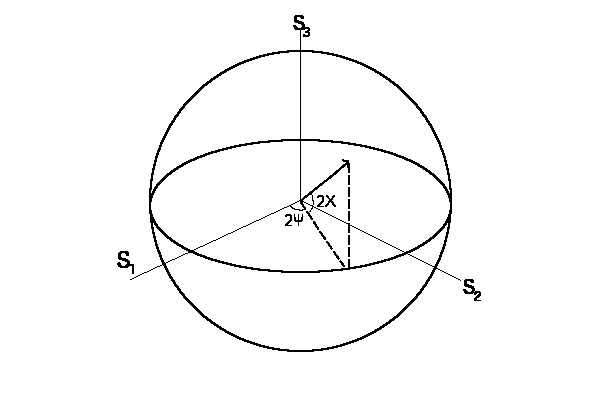
\includegraphics[scale=0.6]{/Sources/Background/Nature_of_Light/POINCARE-binary.png}}
    \end{center}
    \caption{Poincare Sphere}
    \label{fig:polarization}
\end{figure}
%[CHECK]

The zenith angle of the polarization ellipse, represented in Figure as $2\chi$ is found to be related to the parameters of the polarization ellipse by
%
\begin{align}
    sin2\chi = \frac{2E_{0x}2E_{0y}sin\delta}{E_{0x}^2+E_{0y}^2}\qquad -\pi / 4 \leq \chi \leq \pi / 4
\end{align}
%
The azimuth angle $2\psi$ is defined in relation to the parameters of the polarization ellipse as
%
\begin{align}
    tan2\psi = \frac{2E_{0x}2E_{0y}cos\delta}{E_{0x}^2-E_{0y}^2}\qquad 0 \leq \psi \leq \pi
\end{align}
%
For a given state of the polarization ellipse, the angles for plotting the corresponding polarization state on the Poincare sphere can be found using these equations\cite{spieellipse}.

%%%%%%%%%%%%%%%%%%%%%%%%%%%%%%%%%%%%%%%%%%%%%%%%%%%%%%%%%%%
\subsection{Jones Vector Representation}
%%%%%%%%%%%%%%%%%%%%%%%%%%%%%%%%%%%%%%%%%%%%%%%%%%%%%%%%%%%
    %need subsub section on Jones
    % need subsub section on Devices
For the special case of fully polarized EM waves, DOP = 1, the polarization of the beam can be described by a 2x 1 complex vector known as a Jones vector.  The Jones vector relies on the fact that the polarization state of a beam depends only on its relative $X$ and $Y$ intensities, as well as the phase delay between each respective component.

Converting the equation for the electric component of the EM wave into a phasor makes it easy to see the parameters that determine the beam's polarization.  A phasor represents a sinusoidal wave with a constant frequency.  The Jones vectors can be formulated from this representation as
%
\begin{align}
    \underline{\hat{E}}(z)=(\vec{i_x} E_{0x} e^{j\delta_x}+\vec{i_y} E_{0y} e^{j\delta_y })e^{-kz}
\end{align}
%
since the polarization depends on the amplitude and phase difference of the $X$ and $Y$ components, the Jones vector is formally written as
%
\begin{align}
    \underline{J} =
    \begin{bmatrix}
        E_{0x} e^{j\delta_x} \\
        E_{0y} e^{j\delta_y }
    \end{bmatrix}
\end{align}
%
Since only the relative phase differences matter it is common to denote $\delta=\delta_y-\delta_x$.  The vector is also normalized by dividing by its magnitude,
%
\begin{align}
    \underline{J} =
    \frac{1}{\sqrt{E_{0x}^2 + E_{0y}^2}}
    \begin{bmatrix}
        E_{0x} e^{j\delta_x} \\
        E_{0y} e^{j\delta_y }
    \end{bmatrix}
\end{align}
%
An angle can then be defined such that
%
\begin{align}
    tan(\psi) = \frac{E_{0y}}{E_{0x}}
\end{align}
%
The Jones vector can then be written in terms of a single angle
%
\begin{align}
    \underline{J_{\delta}}(\psi) =
    \begin{bmatrix}
        cos(\psi) \\
        sin(\psi)e^{j\delta}
    \end{bmatrix}
\end{align}
%
General states of linear polarization are represented as
%
\begin{align}
    \underline{J_0}(\psi) =
    \begin{bmatrix}
        cos(\psi) \\
        sin(\psi)
    \end{bmatrix}
\end{align}
%
where $\psi$ is any angle in relation to the X axis.  Circular polarization is represented as
%
\begin{align}
    RCP: \underline{J}_{\frac{\pi}{2}} = \frac{1}{\sqrt{2}}
    \begin{bmatrix}
        1 \\
        j
    \end{bmatrix} \\
    LCP: \underline{J}_{-\frac{\pi}{2}} = \frac{1}{\sqrt{2}}
    \begin{bmatrix}
        1 \\
        -j
    \end{bmatrix}
\end{align}
%
\subsubsection{Optical Devices}
Polarization can be naturally occurring, such as in the case of skylight, or it can be created by passing light through an optical device such as a linear polarizer or a quarter wave plate.  Jones vectors are useful for describing the polarization state of an EM wave, while Jones matrices describe nondepolarizing optical devices and the transformation of pure incident polarization states through them.

A linear polarizer is a device that transmits linear polarization states for incident light beams that are aligned with their transmission axis (TA) of the polarizer \cite{polarizedlight}.  For example, if horizontally polarized light is passed through a polarizer with a $TA = 90^{\circ}$, all of the incident light will be extinguished.  In practice all of the light is not completely extinguished and there are often spectral differences to the response of polarizers.

Since linear polarizers block light that is orthogonal to the TA, it can be shown that the general equation for a linear polarizer is such that
%
\begin{align}
    \underline{J}_{in}(\psi + \frac{\pi}{2}) =
    \begin{pmatrix}
        cos(\psi + \frac{pi}{2}) \\
        sin(\psi + \frac{pi}{2})
    \end{pmatrix}
    =
    \begin{pmatrix}
        -sin(\psi) \\
        cos(\psi)
    \end{pmatrix}
\end{align}
%
and
\begin{align}
    \underline{J}_{out} =
    \begin{pmatrix}
        0 \\
        0
    \end{pmatrix}
\end{align}
%
The general equation for Jones interaction with a linear polarizer is
%
\begin{align}
    P(\psi)\underline{J}_{in} = \underline{J}_{out}
\end{align}
\begin{align}
    \begin{pmatrix}
        a & b \\
        c & d
    \end{pmatrix}
    \begin{pmatrix}
        -sin(\psi) \\
        cos(\psi)
    \end{pmatrix}
    =
    \begin{pmatrix}
        0 \\
        0
    \end{pmatrix}
\end{align}
\begin{align}
    -asin(\psi) + bcos(\psi) = 0 \rightarrow atan(\psi) \\
    -csin(\psi) = dcos(\psi) = 0 \rightarrow ctan(\psi)
\end{align}
%
When the incident polarization state is aligned with the polarizers TA, it must also be true that the incident beam goes through the device unchanged.  Therefore,
%
\begin{align}
    \underline{J}_{in}(\psi) =
    \begin{pmatrix}
        cos(\psi) \\
        sin(\psi)
    \end{pmatrix} \\
    \underline{J}_{out}(\psi) =
    \begin{pmatrix}
        cos(\psi) \\
        sin(\psi)
    \end{pmatrix}
\end{align}
\begin{align}
    acos(\psi) + bsin(\psi) = cos(\psi) \\
    ccos(\psi) + dsin(\psi) = sin(\psi)
\end{align}
%
substituting in for previous values of b and d give
%
\begin{align}
    a = \frac{cos(\psi)}{cos(\psi) + tan(\psi)sin(\psi)} = cos^2\psi
\end{align}
\begin{align}
    b = atan(\psi) = sin(\psi)cos(\psi)
\end{align}
\begin{align}
    c = \frac{sin(\psi)}{cos(\psi) + tan(\psi)sin(\psi)} = sin(\psi)cos(\psi)
\end{align}
\begin{align}
    d = ctan(\psi) = sin^2\psi
\end{align}
%
The general form of a linear polarizer with transmission axis angle ? from the X axis is
%
\begin{align}
    P(\psi) =
    \begin{pmatrix}
        cos^2\psi & sin(\psi)cos(\psi) \\
        sin(\psi)cos(\psi) & sin^2\psi
    \end{pmatrix}
\end{align}
%
The intensity of light emerging from a polarizer is governed by Malus law,
%
\begin{align}
    I = I_0cos^2(\theta_i)
\end{align}
%
where $I$ is the intensity of the exiting beam, $I_0$ is the intensity of the incident beam and $\theta_i$ is the angle between the incident polarization state, and the angle of the polarizer.   For incident unpolarized light the equation becomes $I / I_0 = \frac{1}{2}$.  Therefore, the maximum transmittance for an unpolarized beam of light through a polarizer is 50%.  This number is significantly lower for polaroid film based polarizers and can cause potential problems with detector sensitivity for low lighting conditions.

Wave plates create a phase delay between the fast and slow axis of incident linearly polarized light.  Its generalized Jones matrix form can be denoted with a relative phase delay $\delta=\delta_y-\delta_x$,
\begin{align}
    C(\delta) =
    \begin{pmatrix}
        1 & 0 \\
        0 & e^{-j\delta}
    \end{pmatrix}
\end{align}
%
Two common wave plates are the half wave plate and the quarter wave plate.  These produce a delay of $\pi$ and $\pi/2$ respectively.

The noobelectric python package has a module for dealing with these types of problems and it automates Jones optical calculations for purely polarized light beams.  An example for a linear polarizer combined with a quarter wave plate can be created and various input polarization states into the system as shown below.
\begin{lstlisting}
>>> from noobee.jones import j, lp
>>> j_in = j(1,0)
>>> lp_1 = lp(0)
>>> lp_1 * j_in
matrix([[ 1.],
        [ 0.]])
\end{lstlisting}

%%%%%%%%%%%%%%%%%%%%%%%%%%%%%%%%%%%%%%%%%%%%%%%%%%%%%%%%%%%
\subsection{Mueller Matrices}
%%%%%%%%%%%%%%%%%%%%%%%%%%%%%%%%%%%%%%%%%%%%%%%%%%%%%%%%%%%
Interactions with materials that can create depolarization and model partially polarized input and outputs cannot be handled by Jones calculus.  For these problems, Mueller Matrices are used to model the polarization of light with varying degrees of polarization as it interacts with a material.  These interactions are modeled with the equation
\begin{align}
    \mathbf{S}_{out} = \mathbf{M}\mathbf{S}_{in}
\end{align}
%
where
%
\begin{align}
    \mathbf{M} =
    \begin{bmatrix}
        m_{00} & m_{01} & m_{02} & m_{03} \\
        m_{10} & m_{11} & m_{12} & m_{13} \\
        m_{20} & m_{21} & m_{22} & m_{23} \\
        m_{30} & m_{31} & m_{32} & m_{33} \\
    \end{bmatrix}
\end{align}
%
is 4x4 Mueller Matrix that describes the diattenuation, depolarization, and retardance of a materials' polarization response to an input EM beam.

Diattenuation – the two attenuations of orthogonal polarization states [7]

Retardance – the phase difference between two orthogonal polarization states [8]

Depolarization – a process where polarized light becomes unpolarized [8]

It has been shown that these parameters can be found by determining a sample's corresponding Mueller Matrix. The scalar parameters are mathematically defined as,
\begin{align}
    %\emphasis{Diattenuation} = \frac{\sqrt{m_{01}^2 + m_{02}^2 + m_{03}^2}}{m_{00}} \\
%    \emphasis{Retardance} = cos^{-1}(\frac{tr(M_{ret})}{2}-1) \\
%    \emphasis{Depolarization} = 1 - \frac{\sqrt{\sum_{i,j}m_{ij}^2} -m_{00}^2}{\sqrt{3}m_{00}^2}
\end{align}
[TODO explain these equations or remove them]

For nondepolarizing materials, their MM can be converted into Jones matrices.   Examples of Mueller Matrices for common optical elements can be found in [7].  The general form of a linear polarizer with transmission axis at 0 degrees to the $x$ axis is
%
\begin{align}
    \mathbf{M} =
    \begin{bmatrix}
        q + r & q - r & 0 & 0 \\
        q-r & q+r & 0  & 0 \\
        0 & 0 & 2\sqrt{qr} & 0 \\
        0 & 0 & 0 & 2\sqrt{qr}
    \end{bmatrix}
\end{align}
%
where q and r are the attenuation coefficients for the X and Y axis.

%%%%%%%%%%%%%%%%%%%%%%%%%%%%%%%%%%%%%%%%%%%%%%%%%%%%%%
\subsubsection{Mueller Matrix Decomposition}
%%%%%%%%%%%%%%%%%%%%%%%%%%%%%%%%%%%%%%%%%%%%%%%%%%%%%%

The effects of diattenuation, depolarization and retardance can be found to be represented as subsets of the Muller matrix through its decomposition such that the result is
\begin{align}
    \mathbf{M} = m_{00}
    \begin{bmatrix}
        1 & \mathbf{D}^T \\
        \mathbf{P} & \mathbf{m}
    \end{bmatrix}
\end{align}
The derivation of the MM decomposition was made known by Lu and Chipman and is reproduced in [14]. $\mathbf{D}^T$ is the diattenutation vector that describes the amount of decrease in overall polarization for each set of orthogonal polarization states. The m matrix represents the retardance of a material.

$\mathbf{P}$ is the polarizance vector, and describes the amount of light that becomes polarized when unpolarized light is incident.  It is analogous to the effect of depolarization.  This vector can be measured by detecting the output Stokes vector of a material when unpolarized light is incident.  This effect is only evident in materials that create polarization.

%%%%%%%%%%%%%%%%%%%%%%%%%%%%%%%%%%%%%%%%%%%%%%%%%%%%%%%%%%%
\subsection{Reflection and Transmission}
%%%%%%%%%%%%%%%%%%%%%%%%%%%%%%%%%%%%%%%%%%%%%%%%%%%%%%%%%%%

When light interacts with two materials that have different indexes of refraction, the incident beam is reflected and transmitted according to Fresnel’s equations.

The law of reflection states
%
\begin{align}
    \theta_i = \theta_r
\end{align}
%
The transmission is derived directly from Snells equation,
%
\begin{align}
    n_1sin(\theta_i) = n_2sin(\theta_2)
\end{align}
%
Note that part of the transmitted spectra may be absorbed, although this is not considered in these equations.

Two main scenarios are often presented when demonstrating the principles which guide the reflected and transmitted rays; when the incident electromagnetic wave is polarized perpendicular to the plane of incidence, and when the wave is polarized parallel to it.  The perpendicular polarized wave is often denoted S or TE for transverse electric, while the parallel scenario is often denoted P or TM for transverse magnetic.

\begin{figure}[!htb]
    \begin{center}
        \makebox[\textwidth]{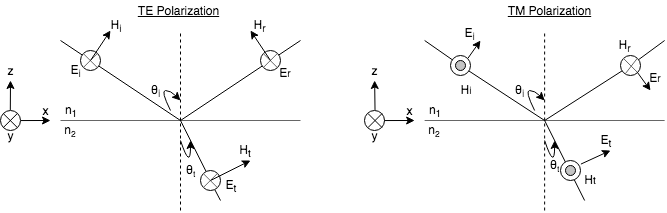
\includegraphics[scale=0.6]{/Sources/Background/Nature_of_Light/fresnel-reflect-trans.png}}
    \end{center}
    \caption{Fresnel Reflection and Transmittance}
    \label{fig:polarization}
\end{figure}

The intensity of the reflected waves for the S and P polarized case are
%
\begin{align}
    \mathbf{R_S} = |\frac{Z_2cos(\theta_i)-Z_1cos(\theta_t)}{Z_2cos(\theta_i)+Z_1cos(\theta_t)}|^2
\end{align}
\begin{align}
    \mathbf{R_P} = |\frac{Z_2cos(\theta_t)-Z_1cos(\theta_i)}{Z_2cos(\theta_t)+Z_1cos(\theta_i)}|^2
\end{align}
%
where Z is the wave impedance for medium 1 and 2.  The power coefficients for transmission are then derived by following the law of conservation of energy such that,
%
\begin{align}
    T_S = 1 - R_S \\
    T_P = 1 - R_P
\end{align}
%
The Brewster angle is a special case where the $P$ polarization state is completely transmitted and no reflection of the TM wave occurs.  The reflected ray is therefore completely $S$ polarized since $R_P$ is zero and $R_S$ is a nonzero intensity.  For perfect air glass interactions typically considered, this angle is approximately 55 degrees.

The Mueller matrix formulation for reflection and transmission reduces to the form of a linear polarizer for ideal surfaces.  It has been shown in \cite{polarizedlight} that the equation for a reflected beam off of a perfectly smooth dielectric surface is
%
\begin{align}
    \begin{split}
    \begin{bmatrix}
        S_{0r} \\
        S_{1r} \\
        S_{2r} \\
        S_{3r}
    \end{bmatrix}
    =
    \frac{1}{2}(\frac{tan(\theta_{-})}{sin(\theta_{+})})^2
    \begin{bmatrix}
       p_S^2 + p_P^2 & p_S^2 - p_P^2 & 0 & 0 \\
        p_S^2 - p_P^2 & p_S^2 + p_P^2 & 0 & 0 \\
        0 & 0 & 2p_Sp_P & 0 \\
        0 & 0 & 0 & 2p_Sp_P
    \end{bmatrix}
    \begin{bmatrix}
        S_0 \\
        S_1 \\
        S_2 \\
        S_3
    \end{bmatrix}
    \end{split}
\end{align}
%
\begin{align}
    p_S = cos^2(\theta_{-}) \\
    p_P = cos^2(\theta_{+})
\end{align}
and $\theta_{\pm}=\theta_i \pm \theta_r$.
This is identical to the form of a linear diattenuator or polarizer from Equation 2.60. For incident unpolarized light the equation simplifies to
%
\begin{align}
    \begin{bmatrix}
        S_{0r} \\
        S_{1r} \\
        S_{2r} \\
        S_{3r}
    \end{bmatrix}
    =
    \frac{1}{2}(\frac{tan(\theta_{-})}{sin(\theta_{+})})^2
    \begin{bmatrix}
        cos^2(\theta_{-}) + cos^2(\theta_{+}) \\
        cos^2(\theta_{-}) - cos^2(\theta_{+}) \\
        0 \\
        0
    \end{bmatrix}
    S_0
\end{align}
%
Therefore, for ideal reflective surfaces, at the Brewster angle, light will be completely polarized perpendicular to the plane of incidence. It should be noted that the case of incident unpolarized light onto the target material, gives the polarizance vector of the Mueller Matrix as described in Section 2.1.3.

Imperfect, non-ideal surfaces have the ability to reflect, transmit and absorb incident electromagnetic radiation.  The outcome of these interactions are related to the physiological makeup of the material, as well as its surface topology.  Multiple scattering mechanisms can be at work within a system, and numerous models have been attempted to balance the tradeoffs between practical realizability for measurements and accurate representation of scattering mechanisms \cite{priest}, \cite{pbrdf}.  Only some of these models attempt to deal with the polarization of the incident, reflected, and transmitted beams.

%%%%%%%%%%%%%%%%%%%%%%%%%%%%%%%%%%%%%%%%%%%%%%%%%%%%%%%%%%%
\subsection{Scattering Mechanisms}
%%%%%%%%%%%%%%%%%%%%%%%%%%%%%%%%%%%%%%%%%%%%%%%%%%%%%%%%%%%

Fresnel’s equations provide an explanation for light reflected and transmitted for ideal surfaces.  This is not the case with most man made and natural materials.  Therefore, more complex mechanisms must be considered when dealing with real world radiation scattering problems.  It has become popular in the field of remote sensing to denote the additional types of interactions as volume scattering and multiple scattering
 interaction.  Single scattering mechanisms are those governed solely by Fresnel’s equations.  The combination of these scattering mechanisms create the diffuse and specular components of reflection.

Single scattering mechanisms create a portion of reflectance known as specular reflectance.  They are often denoted as Type A photons in remote sensing models.  These interactions are highly polarized perpendicular to the plane of incidence as previously discussed. For perfectly smooth dielectrics, this is the dominant scattering mechanism.

Volume scattering occurs when light is absorbed by a material and is readmitted in all directions, including back towards the surface of the material.  They are denoted Type B photons.  Transmittance of this energy back into the first medium obeys the laws of Fresnel’s equations, although the indices of refraction are reversed.  This mechanism accounts for absorption and other higher level light matter interactions, not explained solely by Fresnel’s equations.

Multiple scattering occurs when either Type A or Type B photons interact with the material surface more than once while either being reflected or retransmitted out of the material.  These are denoted Type C photons \cite{schott}.  Figure 2.7 shows each type of interaction.
%
\begin{figure}
    \begin{center}
        \makebox[\textwidth]{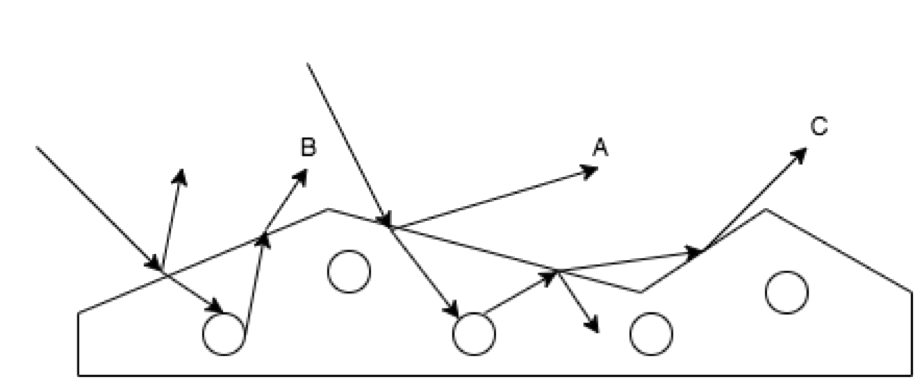
\includegraphics[scale=0.75]{/Sources/Background/Nature_of_Light/photon-interactions-wo.png}}
    \end{center}
    \caption{Various Types of Photon Interactions}
    \label{fig:scattering}
\end{figure}
%
In general type A photons create specular highlights from surfaces that are smooth.  Type B and C photons become more prevalent as a surface becomes rougher.  In most real world applications, surfaces are neither purely specular nor purely diffuse.

Surfaces that are perfectly smooth dielectrics are often considered to be purely specular reflectors of light.  Incident energy is transmitted in an idealized single ray of light from the surface.  Specular reflectors are single scattering mechanisms and result in purely polarized light due to the governance of Fresnel’s equations and are denoted as type A photons.
%
\begin{figure}
    \begin{center}
        \makebox[\textwidth]{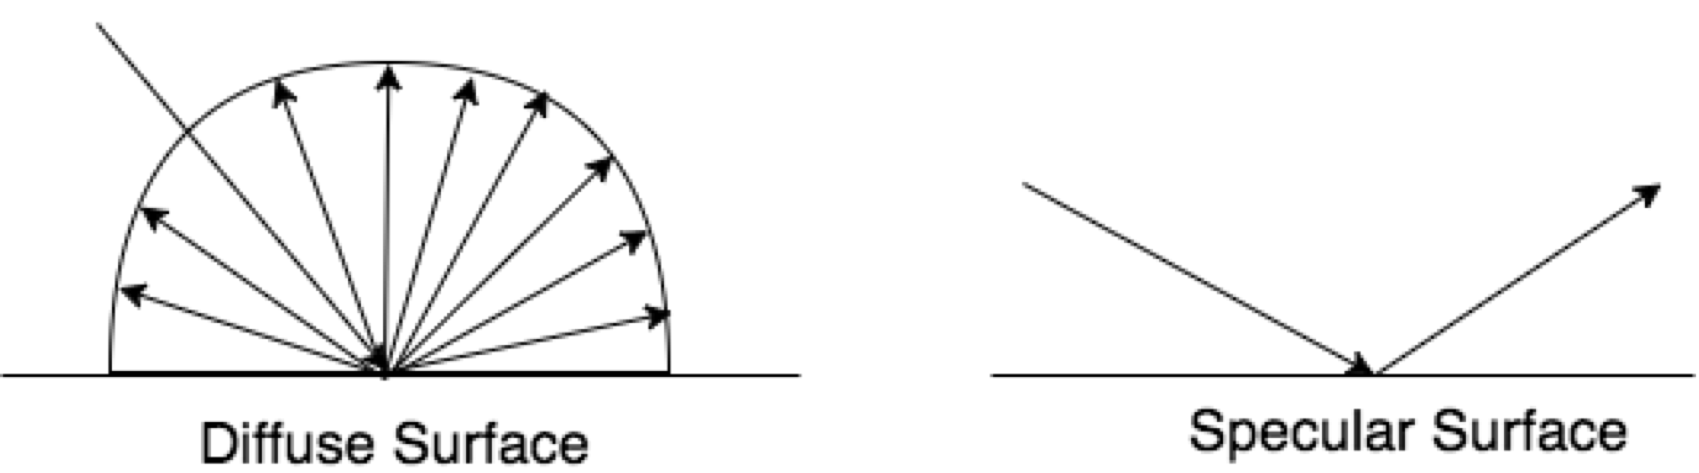
\includegraphics[scale=0.45]{/Sources/Background/Nature_of_Light/diffuse-specular.png}}
    \end{center}
    \caption{Diffuse and Specular Scattering}
    \label{fig:scattering}
\end{figure}
%
In simple models, rough surfaces can be viewed as purely diffuse reflectors that scatter incident light equally in all directions.  Figure 2.8 shows a general example of both specular and diffuse surface scattering.  Perfect diffuse surfaces are known as Lambertian surfaces.  It has been assumed that the diffuse portion of light is unpolarized due to random nature of internal reflections \cite{specularclass}, \cite{grant}.
\begin{figure}
    \begin{center}
        \makebox[\textwidth]{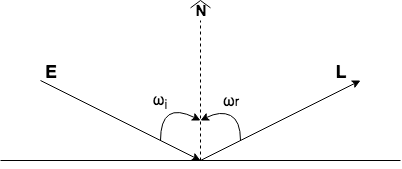
\includegraphics[scale=0.7]{/Sources/Background/Nature_of_Light/brdf-simple.png}}
    \end{center}
    \caption{Simple BRDF Model}
    \label{fig:scattering}
\end{figure}
Bidirectional Reflectance Distribution Functions (BRDF) have been created to model the variety of surface interactions in order to handle the nonideal case where surface roughness is present. BRDFs define how incident radiation is reflected off of opaque surfaces.  It is defined as a ratio of reflected radiance along path $\omega_r$ to incident irradiance $\omega_i$. A simple depiction of this scenario can be found in Figure 2.9.

The BRDF function is often defined in the form
%
\begin{align}
    f_r(\omega_i, \omega_r) = \frac{dL_r(\omega_r)}{dE_i(\omega_i)}[{sr}^{-1}]
\end{align}
%
The units of the BRDF can be reduced from
\begin{align}
    [\frac{dL_r(\omega_r) units}{dE_i(\omega_i) units}] = [\frac{\frac{W}{m^2sr}}{\frac{W}{m^2}}] = [\frac{1}{sr}] = [{sr}^{-1}]
\end{align}
Each $\omega$ is a function of azimuth angle $\phi$ and zenith angle $\theta$. The input irradiance $E$ and output radiance $L$ are measured in units of watts per meter squared and watts per meter squared steradians as shown in Figure 2.10.
where numerous models have been developed for the functions of $L$ and $E$ \cite{sparrow}\cite{brdfoverview}.  In its simplest case the surface is a purely diffuse reflector of incident light and the BRDF becomes
%
\begin{align}
    f_r(\omega_i, \omega_r) = \frac{\rho}{\pi}[{sr}^{-1}]
\end{align}
%
where $\rho$ is the surface albedo, or proportion of light reflected from a surface \cite{nicodemus} and ranges from $0\leq\rho\leq1$.  A general diagram can be found in Figure 2.9.  In the most general case the portion of reflectance that is purely specular can be thought of as a $\delta$ function.  Most surfaces create non-ideal reflections made up of both specular and diffuse components.
%
\begin{figure}
    \begin{center}
        \makebox[\textwidth]{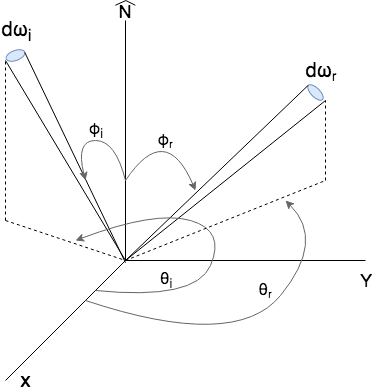
\includegraphics[scale=0.7]{/Sources/Background/Nature_of_Light/brdf-v2.png}}
    \end{center}
    \caption{General BRDF Model}
    \label{fig:scattering}
\end{figure}
%
The notion of a surface being rough, smooth, fine or coarse has been discussed from a perspective of polarized scattering mechanisms. These surface descriptions also come with a connotation of touch and the feel of a materials' surface.  They are textures.


%%%%%%%%%%%%%%%%%%%%%%%%%%%%%%%%%%%%%%%%%%%
\section{Texture and Tone}
%%%%%%%%%%%%%%%%%%%%%%%%%%%%%%%%%%%%%%%%%%%

“When small image areas from black and white photographs are independently processed by a machine, then texture and tone are most important” [4].  Without tone there is no texture, as texture is created when there are certain frequencies of tonal change in an image [12].

A surface texture is classified according to the scale at which the human eye can see.  It is import to determine the appropriate scale for a particular surface, when talking about its texture.  A surfaces ability to appear smooth or rough in an image, is determined by the spatial frequency distribution of grey level pixel intensities in a greyscale image and the various shades of grey tones.  The nature of light reflecting from surfaces of materials is also largely due to the how rough or smooth the surface is.  Imaging devices are able to pick up pixel by pixel surface interactions in their large field of view.  Cameras are able to detect multiple scattering mechanisms for analysis in material classification problems.

Tone is related to texture and is the grey level gradients distributed across an image.  It is the “relative brightness or color of objects on an image” [12].  If an image has no differences in tone, then the texture and other features are indiscernible.

When a pixel is considered as a single color receptor, it represents only tone.  The scaling of the window size to include more pixels allows for texture to become more prevalent.   Scale is important when considering texture since texture is defined in relation to our perception of a materials surface.


%%%%%%%%%%%%%%%%%%%%%%%%%%%%%%%%%%%%%%%%%%%
\subsection{Grey Level Co-Occurence Matrix}
%%%%%%%%%%%%%%%%%%%%%%%%%%%%%%%%%%%%%%%%%%%
A Grey Level Co-Occurrence Matrix (GLCM) is able to quantify the spatial frequency distribution of grey level pixel intensity pairs. The GLCM matrix is formed by determining the frequency of grey level value pixel pairs for a given image.  A relationship is set a priori to determine the direction for grey level comparison.  This relationship is an angle relating a pixel to its neighbor, and is chosen in multiples of either 0 or 45 degrees.  Common GLCM spatial relationships are $0, \pi/4, 3\pi/4, and \pi/2$ radians.
%
\begin{figure}[!htb]
    \begin{center}
        \makebox[\textwidth]{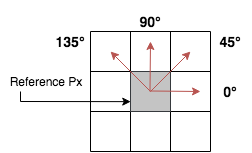
\includegraphics[scale=0.75]{/Sources/Background/Texture_and_Tone/glcm-relationships-no-title.png}}
    \end{center}
    \caption{Defining GLCM Relationships}
    \label{fig:texture}
\end{figure}
%
In order to quantify a texture in a rotationally consistent fashion, all four relationships are usually calculated and averaged together in determining the overall GLCM matrix.  The GLCM has a size of $N x N$ where $N$ is the discrete quantized levels.

A single relationship Co-Occurence matrix is formulated such that,
%
\begin{align}
    \mathbf{\phi}_{ij}(\triangle x,\triangle y) = \sum_{x=0}^{n}\sum_{y=0}^{m}
    \begin{cases}
        1, if I(x,y) = i  and  I(x+\triangle x,y+\triangle y) = j \\
        0, otherwise
    \end{cases}
\end{align}
%
where $I(x,y)$ is an $n x m$ image and $\triangle x,\triangle y$ represent the predefined offset of the grey level pixel neighbor intensity relationship (i,j).
Being defined as referencing one pixel to its neighbor to the right (0 degrees) the GLCM matrix is formulated as such,
%
\begin{figure}[!htb]
    \begin{center}
        \makebox[\textwidth]{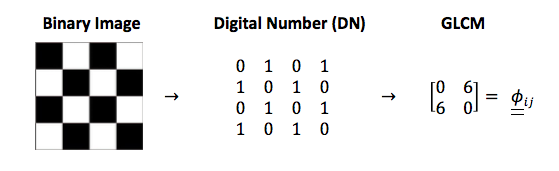
\includegraphics[scale=0.75]{/Sources/Background/Texture_and_Tone/glcm.png}}
    \end{center}
    \caption{Converting a Binary Image to a GLCM Matrix}
    \label{fig:texture}
\end{figure}
%[CHECK]
The example in Figure 2.6 shows the simplest case of a binary image, or an image that only contains white and black pixels.  These pixels values captured by a camera are then converted into there corresponding digital numbers, in this case either zero or one.  With the spatial relationship being defined as one to the right, the GLCM matrix is then formed.

Non symmetrical GLCMs should be symmetrized by adding each to its transpose,
%
\begin{align}
    \mathbf{\phi}^{'} = \mathbf{\phi} + \mathbf{\phi}^{T}
\end{align}
%
Normalizing the frequency to one by dividing the matrix by the sum of all its elements, results in a probability distribution for each grey level pixel pair.
%
\begin{align}
    \mathbf{P} = \frac{\mathbf{\phi}^{'}}{\sum_{i=0}^{N-1}\sum_{j=0}^{N-1}\mathbf{\phi}^{'}}
\end{align}
%
where for the example given above the resulting $\mathbf{P}$ is
%
\begin{align}
    \mathbf{P} = \frac{1}{12}
    \begin{bmatrix}
        0 & 6 \\
        6 & 0
    \end{bmatrix}
    =
    \begin{bmatrix}
        0 & 0.5 \\
        0.5 & 0
    \end{bmatrix}
\end{align}
%
As expected the probability of finding a 0 next to a 1 is the same as finding a 1 next to a zero in a binary checkerboard image.

Features can then be extracted from the formed matrix for the purpose of defining single quantitative values for texture.  These features are known as Haralick features and generally fall into 3 distinct feature categories; Contrast, Statistical and measures of Orderliness \cite{calgary}.

Contrast measures are defined by weights that increase or decrease with distance from the GLCM diagonal.  These weights can be linear, exponential, etc. For the N x N dimensional GLCM matrix the N - 1 term in the first row or column represents pixel relationships that are of the greatest intensity difference.

For example, an 8-bit image has 256 possible grey level values ranging from 0-255, so the maximum amount of contrast occurs when pixel pairs (i,j) are either (0, 255) or (255, 0).

Contrast has weights that increase exponentially away from the diagonal.  It is calculated as
%
\begin{align}
    Contrast = \sum_{i=0}^{N-1}\sum_{j=0}^{N-1}(i-j)^2P_{ij}
\end{align}
%
The dissimilarity is a measure of contrast with weights that increase linearly away from the diagonal
%
\begin{align}
    Diss = \sum_{i=0}^{N-1}\sum_{j=0}^{N-1}|i-j|P_{ij}
\end{align}
%
The dissimilarity of the example binary image can be calculated as
%
\begin{align}
    Diss = \sum_{i=0}^{N-1}\sum_{j=0}^{N-1}|i-j|P_{ij}
    = \sum_{1=0}^{1}|i|P_{i0}+|i-1|P_{i1}
    = 0 + P_{01} + 0 + P_{10} = \frac{1}{3}
\end{align}
%
Statistical measures utilize each individual element of the GLCM as weights to determine the moments of the probability distribution matrix. The mean, variance, correlation, etc. are not measures of individual pixel intensity values, but rather of the intensity of a pixel in relation to its neighbor’s intensity. The mean is the first central moment and is defined by
%
\begin{align}
    \mu_i = \sum_{i=0}^{N-1}\sum_{j=0}^{N-1}iP_{ij} \\
    \mu_j = \sum_{i=0}^{N-1}\sum_{j=0}^{N-1}jP_{ij}
\end{align}
%
Variance is the second moment of the GLCM and is defined as,
%
\begin{align}
    \sigma_i = \sum_{i=0}^{N-1}\sum_{j=0}^{N-1}(i-\mu_i)^2P_{ij}
\end{align}
\begin{align}
    \sigma_j = \sum_{i=0}^{N-1}\sum_{j=0}^{N-1}(j-\mu_j)^2P_{ij}
\end{align}
%
The correlation shows the “linear dependency of grey level values in the Co-Occurence matrix”\cite{haralickcancer}.  It is computed from the values of the variance and mean such that
%
\begin{align}
    Corr = \sum_{i=0}^{N-1}\sum_{j=0}^{N-1}(\frac{(i-\mu_i)(j-\mu_j)}{\sqrt{\sigma_i^2 \sigma_j^2}})
\end{align}
%
If a the GLCM is symmetric, the x and y means and variances are equal and the equations simplify to,
%
\begin{align}
    \mu = \sum_{i=0}^{N-1}\sum_{j=0}^{N-1}iP_{ij}
\end{align}
\begin{align}
    \sigma = \sum_{i=0}^{N-1}\sum_{j=0}^{N-1}(i-\mu)^2P_{ij}
\end{align}
\begin{align}
    Corr = \sum_{i=0}^{N-1}\sum_{j=0}^{N-1}(\frac{(i-\mu)(j-\mu)}{\sigma^2})
\end{align}
%
Measures of orderliness are quantified by the amount of entropy and energy within an image.  Entropy is a measure of randomness in a system.  In thermodynamics, it is the heat lost when a reaction occurs and hence is a measure of disorder.  Energy is a measure of useful work that can occur due to the non random nature of the energy in a system. (clean up this bit on entropy)

The angular second moment (ASM) describes the amount of “inertia” around a pixel neighbor relationship and is defined as,
%
\begin{align}
    ASM = \sum_{i=0}^{N-1}\sum_{j=0}^{N-1}P_{ij}^2
\end{align}
%
The square root of the ASM results in the energy of the system
%
\begin{align}
    Energy = \sqrt{ASM}
\end{align}
%
For perfectly uniform textures the energy will be at a maximum of 1.


%%%%%%%%%%%%%%%%%%%%%%%%%%%%%%%%%%%%%%%%%%%
\section{Plant Physiology}
%%%%%%%%%%%%%%%%%%%%%%%%%%%%%%%%%%%%%%%%%%%
A plant's health is greatly determined by the availability of light, water, and key nutrients in the soil.  These elements are the fundamental inputs to photosynthesis, the process plants utilize to turn light energy into chemical energy for growth.  Nitrogen, Potassium, and Phosphorus are fertilizers (agricultural inputs) that can incur large costs when applied over hectares of farmland, but are needed for healthy plant growth and cell reproduction.

Water is also an essential agricultural input needed for plant photosynthesis and aids in nutrient transport.  Droughts are becoming a global epidemic and precision water management is becoming pivotal for a crops' survival.

The layers of a deciduous leaf contain protection mechanisms, transport systems, and reaction centers for the process of photosynthesis.

%[CHECK insert image of plant layers]
\begin{figure}[!htb]
    \begin{center}
        \makebox[\textwidth]{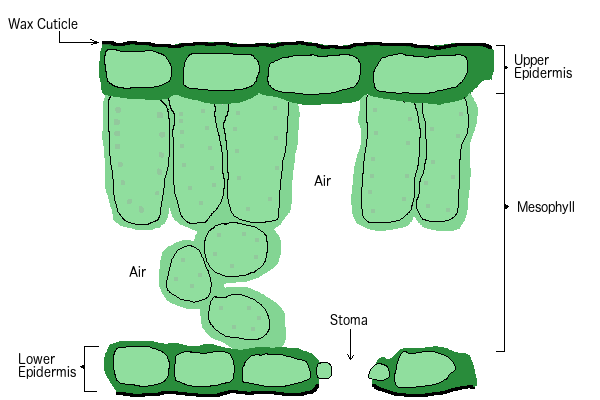
\includegraphics[scale=0.5]{/Sources/Background/Plant_Physiology/leaf-v3.png}}
    \end{center}
    \caption{Major Structures of a Leaf}
    \label{fig:polarization}
\end{figure}

The cuticle wax layer, upper epidermis, and mesophyll layer are the first layers of light interaction on the adaxial surface of the leaf.

The cuticle wax layer provides “the most critical adaptive trait for survival … the ability to retain water in increasingly dehydrating habitats” \cite{cuticle}.  It is the first line of defense for plants and acts as a barrier between water transpiration.

The mesophyll layers contain chloroplasts that convert light energy into chemical energy and consists of two parts. The palisade mesophyll is made up of elongated, organized, compact cells that contain a large number of the chloroplasts.  The spongy mesophyll is irregular in shape and has a large amount of space between its cells to facilitate air and gas exchange [TODO find source].

The upper epidermis consists of very few chloroplasts, and allows most of the light to pass through to the mesophyll layers.


%%%%%%%%%%%%%%%%%%%%%%%%%%%%%%%%%%%%%%%%%%%
\subsection{Photosynthesis}
%%%%%%%%%%%%%%%%%%%%%%%%%%%%%%%%%%%%%%%%%%%

Photosynthesis is a fundamental process that dictates the growth of all land plants.  Water plays an important role in this chemical process, and its availability in plant leaves is an indicator of the plant's ability to perform photosynthesis.

The chemical reaction undergone during photosynthesis involves the conversion of carbon dioxide and water with light energy, to create a carbohydrate and oxygen.  It is formally written as,
%
\begin{align}
    6CO_2 + 6H_2O \xrightarrow{\text{light}} C_6H_12O_6 + 6O_2
\end{align}
%
Due to water's integral role in this reaction, water stress in plants can lead to decreased photosynthetic activity.  It was pointed out by Ehleringer, referenced in \cite{akinci}, that water stress “can decrease…photosynthesis by reflecting quanta that might have been used in photosynthesis”.   Chlorophyll is an essential pigment in photosynthesis due to it being “an efficient light-absorbing molecule” \cite{ecophysiology}.  It is highly absorbing in the blue and red spectrum of visible light, and more reflective in the green portion.  The absorption spectrum for chlorophyll can be found in \cite{chemistry}. This spectrum is what causes many leaves to appear green.  Note that is regions outside the visible, chlorophyll does not absorb the incident radiation.

%%%%%%%%%%%%%%%%%%%%%%%%%%%%%%%%%%%%%%%%%%%
\subsection{Relative Water Content}
%%%%%%%%%%%%%%%%%%%%%%%%%%%%%%%%%%%%%%%%%%%
The Relative Water Content (RWC) of a leaf is a measure of the current water level based on the total leaf water retaining capacity.  It is a useful measure of the water balance within a plant as it expresses the absolute amount of current water in a plant, in proportion to the minimum amount of water it can hold.

Water makes up over 90\% of the mass of a leaf, and although RWC provides a good indicator of plant health and water capacity, it is highly dependent on the age and maturity of the leaf.  It should also be taken into consideration that leaves can also be very heterogeneous and contain a variety of complex structures in different stages of growth, within each individual leaf.

Correlations between the RWC and other physiological responses have been found in [9].

\begin{table}[h]
  \centering
  \begin{tabular}{ll}
    \toprule
    \textbf{Relative Water Content ~(\%)}      & \textbf{Plant Physiological Response}\\
    \midrule
      \texttt{90-100}          & closing of the stomata, reduction of cellular expansion and growth\\
      \texttt{80-90}           & tissue composition change, altered rates of photosynthesis and respiration\\
      \texttt{<80}         & ceasing of photosynthesis\\
    \bottomrule
  \end{tabular}
  \caption{%
    Plant physiological responses to detected relative water content levels.
  }
  \label{tab:Packages}
\end{table}

“An increase in reflectance…is not directly related to water content but indirectly, since a decrease in water content can lead to an increase in internal lead air space or cell breakdown which may increase reflectance and decrease transmittance [2]”.

This increase in internal air space leads to multiple scattering at air wax boundaries, and creates differences in the reflection and transmission of light, absorption, and the $S1$ and $S2$ Stokes parameters of the polarization response.

Field measurements of the physiological properties of plants are time consuming and error prone.  It is therefore beneficial to pursue solutions to quantifying these metrics in large area field measurements.


%%%%%%%%%%%%%%%%%%%%%%%%%%%%%%%%%%%%%%%%%%%
\section{Remote Sensing of Vegetation}
%%%%%%%%%%%%%%%%%%%%%%%%%%%%%%%%%%%%%%%%%%%

%%%%%%%%%%%%%%%%%%%%%%%%%%%%%%%%%%%%%%%%%%%
\subsection{Vegetation Indices and Spectral Responses}
%%%%%%%%%%%%%%%%%%%%%%%%%%%%%%%%%%%%%%%%%%%
Spectral response patterns in remote sensing have been shown to useful [many sources] for determining the health of land vegetation.  The reflection and scattering of light off vegetation using different spectral bands of incident light, allows for the classification of land objects and vegetation health.  The detector response to these processes are known as spectral responses.  Spectral responses are quantitative measures that change with the condition of the vegetation under inspection.  As plants become stressed, as in the case of water deficiency or drought, their physiological makeup changes.  A variety of different factors can affect the exact spectral response of an object [12].

Vegetative Indices (VI) are ratios between different spectral responses for the purpose of determining the condition and health of plants.  Various combinations of frequencies have been combined to form standard VI’s utilizing the visible spectrum and the infrared spectrum. In its most basic form a vegetation index is defined by,
%
\begin{align}
    VI = Ch1 - Ch2
\end{align}
%
where Ch1 and Ch2 are the channels of the detected spectral responses.

The Normalized Difference Vegetation Index (NDVI) utilizes a plant's response to Near Infrared and Visible Red energy.  This is a measure of the chlorophyll content within the leaves since the leaf is highly reflective and transmissive in the NIR since plants cannot use light outside of the visible spectrum for photosynthesis.  This band represents the amount of cellulose contained within the plant.  The red light is used by chlorophyll for photosynthesis.  It also interacts with the cell wall and is therefore a measure of both chlorophyll content and cellulose.  The difference between these two spectral responses is the NDVI.
%
\begin{align}
    NDVI = \frac{NIR - VIS_{red}}{NIR + VIS_{red}}
\end{align}
%
In comparison, clouds, snow, and water all have relatively high visible responses and low NIR response.  Therefore, little interference from these effects is contributed to the overall NDVI.  Moreover, most satellites average NDVI recordings over a few days to also alleviate any interference with clouds and other particles in the atmosphere [12].
The NDVI takes advantage of the extreme shift in reflectance and transmittance for plants between the visible and near infrared regions known as the red gap shown in Figure 10.

%TODO insert transmittance and reflectance image

The reflectance curve for a plant leaf versus wavelength, shows that green light (~500-600nm) is the most reflected wavelength of light, and accounts for the green color of leaves. Red is (~600-750nm) and and blue light (~400-500nm) are shown to be highly absorbed.  This is due to these frequencies being used in photosynthesis and the high absorption of chlorophyll in these regions.

It should also be noted that as leaves dry down and become brown in color, the reflectance curve in the red part of the spectrum greatly increases [photon vegetation].  The magnitude of this change is dependent on the species of plant, as well as the maturity of the individual leaf structures.

There are also metrics that utilize the visible spectrum such as the Visible Atmospherically Resistant Index (VARI) [13].  It is defined as
%
\begin{align}
    VARI = \frac{VIS_{green} - VIS_{red}}{VIS_{green} + VIS_{red}-VIS_{blue}}
\end{align}
%
The vegetation indices described, all indirectly describe the amount of photosynthetic activity occurring within the plant.  They are sensitive to the local growing conditions, growth stage of plants, and other factors. The major spectral responses of pigments within plants have been studied in vivo in order to gain insight into how light is utilized on a metabolic level by plants, in the process of photosynthesis.

%%%%%%%%%%%%%%%%%%%%%%%%%%%%%%%%%%%%%%%%%%%
\subsection{Reflection and Transmission of Light and Leaves}
%%%%%%%%%%%%%%%%%%%%%%%%%%%%%%%%%%%%%%%%%%%

The reflectance of light off of a leaf is dependent on many different factors.  As plants undergo stressful conditions, there reflectance and transmittances change.  In general, as photosynthetic activity decreases, the reflection off of the surface increases.  As a results there is also less transmission.  The growth stage of the leaf is also import as younger leaves have not fully developed all of the internal complex structures.  As the number of complex structures increases, there is an increase in the number of air wax interfaces to cause more randomized reflection and refraction [2].

Leaves that succumb to disease also may become deformed and further alter the response recorded from the canopy layer.

It has been shown [26, 30] that leafs are not purely diffuse or purely specular reflectors of light.  There response is best modelled as a combination of both components.

%%%%%%%%%%%%%%%%%%%%%%%%%%%%%%%%%%%%%%%%%%%
\subsection{Polarization of Light from Leaves}
%%%%%%%%%%%%%%%%%%%%%%%%%%%%%%%%%%%%%%%%%%%

An increase in the reflectance of light off the surface of a leaf, as it reflects wavelengths it would normally use for photosynthesis, allows for the polarization response of the leaf to be observed.  As stated in [2] “Polarization provides the capability to separate light scattered by the leaf mesophyll from light scattered by the air-cuticle surface”.  Specular reflections, that occur at the Brewster angle provide information on the topology of leaf surfaces.  Leaves are not optically smooth and therefore the typical application of Fresnel’s equations for reflection and transmission must be extended to handle rough surfaces. A pBRDF [TODO explain this model] model adapted for leaf surfaces can be found in [2].

The specular component is sometimes so bright that it can make an entire canopy appear white to the observer.  This portion is usually highly polarized and tells of the surface topology of the leaves [31].  The diffuse component is often assumed to be randomly polarized, although our results show there is potential to discriminate with diffuse polarization.

%%%%%%%%%%%%%%%%%%%%%%%%%%%%%%%%%%%%%%%%%%%
\subsection{Classification of Vegetation Species}
%%%%%%%%%%%%%%%%%%%%%%%%%%%%%%%%%%%%%%%%%%%
In addition to determining the relative health of vegetation, remote sensing can be useful to classify fields' and canopies' heterogeneous combination of species.  The spectral characteristics of each pixel in an acquired image can be combined into similar groups for classification and is known as spectral pattern recognition.

Pixel relationships that represent texture, feature size, etc. can also be used for classification and is known as spatial pattern recognition. This method is often computationally more intensive than its spectral counterpart, as additional calculations need to be performed in order to extract this information.

A hybrid approach can also be used, which combines both spectral and spatial response patterns for the purpose of classifying image scenes.

Challenges to this include the variation of vegetation with different seasons, health status and growth stage.


